\section{2. Time-Independent Schr\"{o}dinger Equation} \hrule height 0.3pt \thinspace

\subsection{\underline{2.1 Stationary States}}
Suppose PE is independent of time, $V(\vec{r}, t) = V(\vec{r})$. \\
Separation of variables: $\Psi(\vec{r}, t) = \psi(\vec{r}) \varphi(t)$ \\

Eq of motion for $\varphi(t)$: $\varphi(t) = e^{-iEt/\hbar}$ \\

Eq of motion for $\psi(\vec{r})$ is the TISE:
$-\frac{\hbar^2 }{2m} \dv[2]{\psi(\vec{r})}{x} + V(\vec{r}) \psi(\vec{r}) = E \psi(\vec{r}) $

TD of the wavefunction that corresponds to the constant $E$ is easily written once we solve the TISE: $\Psi_{E}(\vec{r}, t) = \psi_{E}(\vec{r}) e^{-iEt / \hbar}$

\hrule height 0.06pt

Properties of solutions for TI potentials:

\vspace{-10pt}

\begin{itemize}[noitemsep,wide=0pt, leftmargin=\dimexpr\labelwidth + 2\labelsep\relax]
    \item \textbf{The constant $E$ must be real.}
    
    \item \textbf{Stationary wavefunction.}
        $\mathcal{P}(\vec{r}, t) = |\psi_E(\vec{r}, t)|^2 = |\psi_E(\vec{r})|^2$ (TD cancels).

    \item \textbf{Stationary wavefunction is a state of definite energy.} \\
        Total E (kinetic + potential) is the Hamiltonian: $H(x, p) = \frac{p^2}{2m} + V(x)$

        Hamiltonian operator: $\widehat{H} = -\frac{\hbar^2}{2m} \pdv[2]{}{x} + V(x)$.
        TISE: $\widehat{H} \psi = E \psi$ \\

        $\langle \widehat{H} \rangle = E$, $\langle \widehat{H} ^2 \rangle = E^2$, $\Delta E = \sqrt{\langle \widehat{H}^2 \rangle - \langle \widehat{H} \rangle ^2} = 0$

    \item \textbf{Spatial part of stationary wavefunction can be chosen to be real.} \\
        $\psi^*(\vec{r})$ is a soln w/ same $E$ \\
        Solns can be chosen to be real: $\psi(\vec{r}) + \psi^*(\vec{r})$ and $\frac{\psi(\vec{r}) - \psi^*(\vec{r})}{i}$.

    \item \textbf{Parity symmetry: even and odd wavefunctions.}
        Suppose $V(-\vec{r}) = V(\vec{r})$. Then, $\psi_E(-\vec{r})$ is a soln w the same energy. \\
        $\psi_E(\vec{r}) + \psi_E(-\vec{r})$ is even under reflection, $\psi_E(\vec{r}) - \psi_E(-\vec{r})$ is odd. \\
        When the potential is symmetric under reflection, we can choose the stationary states to be either even or odd under reflection.

    \item \textbf{Orthogonality/orthonormality.} \\
        $\int \psi_m (\vec{r})^* \psi_n (\vec{r}) d^3 \vec{r} = \delta_{mn}$ where $\delta_{mn}$ is 0 if $m \neq n$ and 1 if $m = n$.

    \item \textbf{Linearity.} \\
        The SE is linear. Given stationary states, a linear combo of these
            $$\psi(\vec{r}, t) = \sum_{n} c_n \psi_n(\vec{r}, t) = \sum_n c_n \psi_n(\vec{r}) e^{-\frac{i}{\hbar} E_n t}$$
        where $c_n$ are complex constants, is a soln the TDSE 
        $i \hbar \pdv{\psi(\vec{r}, t)}{t} = \widehat{H} \psi(\vec{r}, t)$

    \item \textbf{Time evolution.}
        Given $\psi(\vec{r}, 0) = \sum_n c_n \psi_n(\vec{r}, 0) = \sum_n c_n \psi_n (\vec{r})$
        at time $t$, the time evolution is 
        $\psi(\vec{r}, t) = \sum_n c_n \psi_n(\vec{r}, t) = \sum_n c_n \psi_n(\vec{r}) e^{-\frac{i}{\hbar} E_n t}$

        Once we've expanded a given initial wavefunction in terms of a linear combo of the stationary wavefunctions $\psi_n(\vec{r})$, the time evolution follows simply by putting a factor of $e^{-i/\hbar E_n t}$ to each term containing $\psi_n(\vec{r})$.

    \item \textbf{Normalization.}
        The constant coefficients are constrained by $\sum_n |c_n|^2 = 1$

    \item \textbf{Completeness.}
        The stationary states form a complete set if $\sum_n \psi_n (\vec{r'}, t)^* \psi_{n} (\vec{r}, t) = \delta^3 (\vec{r'} - \vec{r})$, where $\delta^3(\vec{r'} - \vec{r})$ is the Dirac-delta function in 3D defined by $\int d^3 \vec{r'} \psi(\vec{r'}, t) \delta^3(\vec{r'} - \vec{r}) = \psi(\vec{r}, t)$
\end{itemize}

\vspace{-10pt}

\textbf{Euler's formula}: $e^{i \theta} = \cos \theta + i \sin \theta$ \\
\textbf{sin and cos}: $\cos(\theta) = \frac{1}{2}(e^{i \theta} + e^{-i \theta})$, $\sin(\theta) = \frac{1}{2}(e^{i \theta} - e^{-i \theta})$ \\

%\textbf{Delta function}: Given $f(x)$, $\delta(x - x')$ is defined as $f(x') = \int f(x) \delta(x - x') dx$ \\
%$\int \delta(x - x') dx = 1$, note this is not the area \\

%    $\delta_{\alpha}(x) = \frac{1}{\alpha \sqrt{\pi}} e^{-\frac{x^2}{\alpha^2}}$,
%    $\delta_{\alpha}(x) = \frac{1}{\pi x} \sin(\frac{x}{a})$, 
%    $\delta_{\alpha}(x) = \frac{\alpha}{\pi x^2} \sin^2 (\frac{x}{\alpha})$ \\

\subsection{\underline{One-dimensional systems}}
Wavefunction for a system containing a single particle of mass $m$ in 1D with TI potentials.
    $- \frac{\hbar^2}{2m} \dv[2]{\psi(x)}{x} + V(x) \psi(x) = E \psi(x)$

Time dependence: $\psi_E(x, t) = \psi_E(x) e^{-\frac{i}{\hbar} E t}$

\textbf{Boundary conditions} \\
1. When the potential $V(x)$ has a finite jump at $x = a$, both $\psi(x)$ and $\psi'(x)$ are continuous across $x = a$. \\
2. When the potential $V(x)$ has an infinite jump at $x = a$, $\psi(x)$ is continuous but $\psi'(x)$ is discontinuous across $x = a$.

Wavefunction must vanish at $x = \pm \infty$ to be normalizable.

\subsection{\underline{2.2 The Infinite Square Well}}

$V(x) = \left\{ 0 \textrm{ if } 0 \leq x \leq a; \quad \infty \textrm{ otherwise} \right\}$

%\begin{align*}
%    V(x) = 
%        \begin{cases} 
%            0, & \textrm{if } 0 \leq x \leq a \\
%            \infty, & \textrm{otherwise}
%        \end{cases}
%\end{align*}

$\psi(x) = 0 \textrm{ for } x < 0 \textrm{ and } x > a$
For $0 \leq x \leq a$, $V(x) = 0$. The SE: 
    $$\psi''(x) + k^2 \psi(x) = 0 \textrm{, where } k = \sqrt{\frac{2mE}{\hbar^2}} \textrm{ and } E > 0$$

Classic \textbf{simple harmonic oscillator}: $\psi(x) = A \sin(kx) + B \cos(kx)$ \\

\textbf{Boundary conditions}: \\
Continuity of $\psi(x)$ at $x = 0$ sets $\psi(0) = B = 0 \rightarrow \psi(x) = A \sin(kx)$ \\
at $x = a$ sets $\psi(a) = A \sin(ka) = 0$

$$k_n = \frac{n \pi}{a}, n = 1,.. \quad \psi_n(x) = \sqrt{\frac{2}{a}} \sin(\frac{n \pi}{a} x) \quad E_n = \frac{\hbar^2 k_n^2}{2m} = \frac{n^2 \pi^2 \hbar^2}{2ma^2}$$

%$\psi_1$ is the ground state, others are excited states. \\

%Properties of $\psi_n(x)$: \\
%1. Alternatively even and odd. \\
%2. As you go up in energy, each successive state has one more node. \\
%3. They are mutually orthogonal, in the sense that $\int \psi_m(x)* \psi_n(x) dx = 0$ whenever $m \neq n$. \\

%$\int \psi_m (x)* \psi_n(x) dx = \delta_{mn}$
%where $\delta_{mn}$ (Kronecker delta) is 0 if $m \neq n$ and 1 if $m=n$. We say that the $\psi$'s are orthonormal.

They are complete, in the sense that any other function, $f(x)$, can be expressed as a linear combination of them (Fourier series), Dirichlet's theorem:
    $$f(x) = \sum_{n=1}^{\infty} c_n \psi_n(x) = \sqrt{\frac{2}{a}} \sum_{n=1}^{\infty} c_n \sin(\frac{n \pi}{a} x)$$

Fourier's trick: $c_n = \int \psi_n(x)^* f(x) dx$
$$c_m = \frac{2}{a} \int_0^a f(x) \sin(\frac{m \pi x}{a}) dx$$

$|c_n|^2$: probability that a measurement of the energy would yield the value $E_n$. \\

Sum of these probabilities should be 1: $\sum_{n=1}^{\infty} |c_n|^2 = 1$

The expectation value of the energy is $\langle H \rangle = \sum_{n=1}^{\infty} |c_n|^2 E_n$

\subsection{\underline{2.3 The Harmonic Oscillator}}
Hooke's law (mass $m$ w/ spring constant $k$): $F = -kx = m \frac{d^2 x}{d t^2}$ \\
Solution is $x(t) = A \sin(\omega t) + B \cos(\omega t)$, where $\omega = \sqrt{\frac{k}{m}}$ \\
Potential energy: $V(x) = \frac{1}{2} k x^2 = \frac{1}{2} m \omega^2 x^2$ \\

Expanding $V(x)$ in a \textbf{Taylor series} about the min: $V(x) = V(x_0) + V'(x_0) (x - x_0) + \frac{1}{2} V''(x_0)(x- x_0)^2 + \cdots$ \\
Simple harmonic oscillaton, $V(x) \cong \frac{1}{2} V''(x_0) (x - x_0)^2, k = V''(x_0)$

SE for the harmonic oscillator: $-\frac{\hbar^2}{2m} \dv[2]{\psi}{x} + \frac{1}{2} m \omega^2 x^2 \psi = E \psi$

Boundary conditions: $\psi(-\infty) = 0, \qquad \psi(+\infty) = 0$

\smallskip

\textit{\underline{1. Simplify notation with change of variables}} \\
Introduce $\xi \equiv \sqrt{\frac{m \omega}{\hbar}} x$.
SE becomes $\dv[2]{\psi}{\xi} = (\xi^2 - K) \psi$, where $K \equiv \frac{2E}{\hbar \omega}$. \\

\textit{\underline{2. Asymptotic behavior}} \\

Working in the large $\xi^2 >> K$ region, \\
\textbf{Hermite eqn}: $H''(\xi) - 2 \xi H'(\xi) + (K - 1) H(\xi) = 0$ \\

\textbf{Hermite polynomials}: $H_0 = 1$, $H_1 = 2 \xi$, $H_2 = 4 \xi^2 - 2$, $H_3 = 8 \xi^3 - 12 \xi$, $H_4 = 16 \xi^4 - 48 \xi^2 + 12$, $H_5 = 32 \xi^5 - 160 \xi^3 + 120 \xi$ \\

\textit{\underline{3. Method of power series}}

%\begin{vwcol}[widths={0.7,0.3},sep=.1cm,rule=0pt,indent=0em]

Recursion: $a_{j+2} = \frac{(2j + 1 - K)}{(j + 1)(j + 2)} a_j$. For allowed $K$: $a_{j+2} = \frac{-2(n - j)}{(j+1)(j+2)} a_j$ \\

$h(\xi) = a_0 + a_1 \xi + a_2 \xi^2 + \cdots = \sum_{j=0}^{\infty} a_j \xi^j$,
$h(\xi) = h_{\text{even}}(\xi) + h_{\text{odd}}(\xi)$ \\

%\columnbreak

%\vspace{-1em}
%\begin{Figure}
%    \raggedright
%    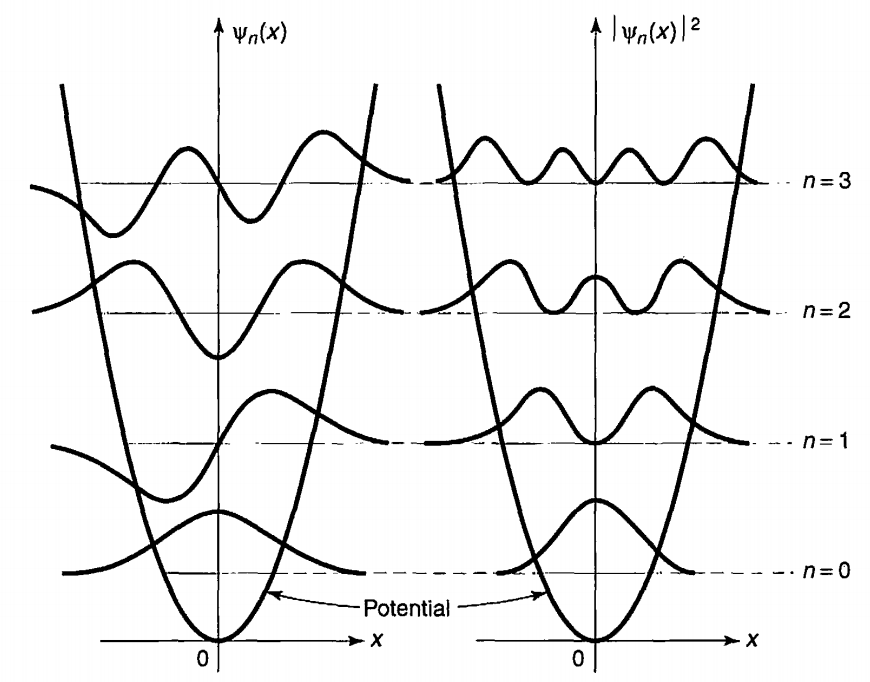
\includegraphics[width=0.3\columnwidth]{figures/harmonic_oscillator1.png}
%\end{Figure}
%\vspace{-1em}

%\end{vwcol}

\textit{\underline{4. Infinite series produces a diverging function}}
For large $n$, $a_{n+2} \approx \frac{2}{n} a_n$ 

\textit{\underline{5. Truncate series}} $K = 2n + 1$, so $E_n = (n + \frac{1}{2}) \hbar \omega$

Normalized stationary states:
$\psi_n(x) = (\frac{m \omega}{\pi \hbar})^{1/4} \frac{1}{\sqrt{2^n n!}} H_n(\xi) e^{-\xi^2 / 2}$ \\

Rodrigues formula: $H_n(\xi) = (-1)^n e^{\xi^2} (\dv{}{\xi})^n e^{-\xi^2}$

%\columnbreak

%\vspace{-1em}
%\begin{Figure}
%    \raggedright
%    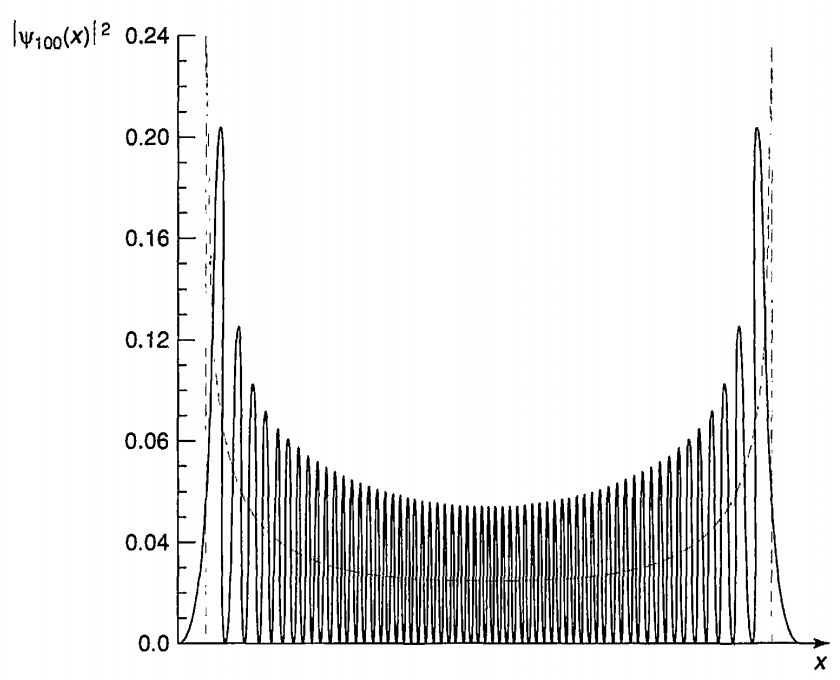
\includegraphics[width=0.2\columnwidth]{figures/harmonic_oscillator2.png}
%\end{Figure}
%\vspace{0em}

%\end{vwcol}

\subsection{\underline{2.4 The Free Particle}}
$E > V(x)$ for all $x$, $V(x) = 0, -\infty < x < \infty$ \\

We have $x(t) = v_{cl} t$, where $v_{cl}$ is the classical velocity of the particle.

$\psi''(x) + k^2 \psi(x) = 0, k \equiv \sqrt{\frac{2mE}{\hbar^2}}$ \\
$\Psi(x, t) = Ae^{ikx - i \frac{\hbar k^2}{2m} t} + Be^{-ikx - i \frac{\hbar k^2}{2m} t} = A e^{i(kx - wt)} + Be^{-i(kx + \omega t)} = A e^{ik(x - v_p t)} + Be^{-ik(x + v_{p} t)}$,
where $\omega = \frac{E}{\hbar} = \frac{\hbar k^2}{2m}$ is angular vel, $v_p = \frac{\omega}{k} = \frac{\hbar k }{2m} = \frac{p}{2m} = \frac{1}{2} v_{cl}$ is phase velocity. \\

Not normalizable. General sol to the TISE: wave packet, 
\tiny
$\Psi(x, t) = \frac{1}{\sqrt{2\pi}} \int_{-\infty}^{\infty} \phi(k) e^{i (kx - \frac{\hbar k^2}{2m} t)} dk$,
$\phi(x) = \frac{1}{\sqrt{2 \pi}} \int_{-\infty}^{+\infty} \Psi(x, 0) e^{-ikx} dx$
\scriptsize

$$f(x) = \frac{1}{\sqrt{2 \pi}} \int_{-\infty}^{\infty} F(k) e^{ikx} dk \leftrightarrow F(k) = \frac{1}{\sqrt{2\pi}} \int_{-\infty}^{\infty} f(x) e^{-kx} dx$$

$F(k)$ is Fourier transform of $f(x)$; $f(x)$ is inverse Fourier transform of $F(k)$ \\

%Phase velocity: speed of individual ripples; group velocity: speed of the envelope \\

%Dispersion relation: the formula for $\omega$ as a function of $k$

\subsection{\underline{2.5 The Delta-Function Potential}}

\textbf{Dirac delta function}, area is 1:
$\delta(x) = \left\{ 0, \textrm { if } x \neq 0; \quad \infty, \textrm{ if } x = 0 \right\}$
%\begin{align*}
%    \delta(x) = 
%        \begin{cases} 
%            0, & \textrm{if } x \neq 0 \\ 
%            \infty, & \textrm{if } x = 0 
%        \end{cases}
%\end{align*}

$f(x) \delta(x - a) = f(a) \delta(x - a)$ bc the product is 0 anyway except at $a$. \\

In particular, $\int_{-\infty}^{\infty} f(x) \delta(x-a) dx = f(a)$

$V(x) = -\alpha \delta(x)$, where $\alpha$ is positive constant. $-\frac{\hbar^2}{2m} \dv[2]{\psi}{x} - \alpha \delta(x) \psi = E \psi$

\underline{$\textit{Bound states } (E < 0)$:} \\

\textbf{REGION I}, $x < 0, V(x) = 0$ \\
$\dv[2]{\psi_{I}}{x} - \kappa^2 \psi_{I} = 0$, where $\kappa \equiv \frac{\sqrt{-2mE}}{\hbar}$. \\

General sol: $\psi(x) = Ae^{-\kappa x} + Be^{\kappa x}$
But $A = 0$, so $\psi(x) = Be^{-\kappa x}, (x < 0)$.

\textbf{REGION II}, $x > 0, V(x) = 0$
$\psi(x) = Fe^{-\kappa x} + Ge^{\kappa x}$ \\
But $G = 0$, so $\psi(x) = Fe^{-\kappa x}, (x > 0)$.

The first boundary condition tells us that $F=B$, so

$\psi(x) = \left\{ Be^{\kappa x}, (x \leq 0), \qquad Be^{-\kappa x}, (x \geq 0) \right\}$

%\begin{align*}
%    \psi(x) = 
%    \begin{cases}
%        Be^{\kappa x}, & (x \leq 0), \\
%        Be^{-\kappa x}, & (x \geq 0) 
%    \end{cases}
%\end{align*}

The discontinuity of $\psi'(x)$ across $x=0$ follows from 
\begin{align*}
    \psi'_{II}(0) - \psi'_{I}(0) 
    &= \lim_{\epsilon \rightarrow 0} \int_{-\epsilon}^{\epsilon} \psi''(x) dx = \lim_{\epsilon \rightarrow 0} \int_{-\epsilon}^{\epsilon} \frac{2m}{\hbar^2} (V(x) - E) \psi(x) dx \\
    &= - \frac{2m}{\hbar^2} \int_{-\epsilon}^{\epsilon} \alpha \delta(x) \psi(x) dx = \frac{2m}{\hbar^2} \alpha \psi(0) = - \frac{2m}{\hbar^2} \alpha F
\end{align*}

Taking the derivatives directly, $\psi'_{II}(0) - \psi'_{I}(0) = -\kappa F - \kappa B$. Therefore,
    $\kappa F + \kappa B = \frac{2m}{\hbar^2} \alpha F \rightarrow \kappa = \frac{m \alpha}{\hbar^2} \rightarrow E = - \frac{m \alpha^2}{2 \hbar^2}$

Only one $E$, so only one bound state.

Normalizing: $1 = \int_{-\infty}^{0} B^2 e^{2 \kappa x} + \int_{0}^{\infty} B^2 e^{-2 \kappa x} = B^2 \frac{1}{2 \kappa} + B^2 \frac{1}{2 \kappa} = \frac{B^2}{\kappa}$, which gives $B = \sqrt{\kappa}$. \\

The normalized wavefunction is: 
\begin{align*}
\psi(x) = 
    \begin{cases} 
        \sqrt{\kappa} e^{-\kappa x} = \sqrt{\frac{m\alpha}{\hbar^2}} e^{-\frac{m\alpha}{\hbar^2}} x, & x > 0 \\ 
        \sqrt{\kappa} e^{\kappa x} = \sqrt{\frac{m\alpha}{\hbar^2}} e^{\frac{m \alpha}{\hbar^2}} x, & x < 0
    \end{cases}
\end{align*}

\underline{$\textit{Scattering states } (E > 0) \textit{ -- reflection and transmission}$:} \\

For $x < 0$ the SE reads $$\dv[2]{\psi}{x} = -\frac{2mE}{\hbar^2} \psi = -k^2 \psi, \qquad k \equiv \frac{\sqrt{2mE}}{\hbar}$$

General sol is $\psi(x) = Ae^{ikx} + Be^{-ikx}$ \\
For $x > 0$, $\psi(x) = Fe^{ikx} + Ge^{-ikx}$ \\

Continuity of $\psi(x)$ at $x = 0$: $F+G=A+B$ \\

Reflection coefficient: $R \equiv \frac{|B|^2}{|A|^2}$, 
Transmission coefficient: $T \equiv \frac{|F|^2}{|A|^2}$ \\
$R + T = 1$, $R = \frac{1}{1+(2\hbar^2E/m \alpha^2)}, T = \frac{1}{1+m \alpha^2 / 2 \hbar^2 E)}$ \\
Higher $E \rightarrow$ greater probability of transmission.

\subsection{\underline{Step potential}}
Particle of energy $E > V_0$ approaching a step potential from the left in the $x < 0$ region with $V(x) = \left\{ 0, x < 0; \quad V_0, x > 0 \right\}.$ \\

Incident and reflected waves in region $I$, only transmitted wave in region $II$:
$\psi_{I}(x) = Ae^{ikx} + Be^{-ikx}, \quad \psi_{II}(x) = Ce^{i\kappa x}$ \\
where $k = \sqrt{\frac{2mE}{\hbar^2}}, \kappa = \sqrt{\frac{2m(E - V_0)}{\hbar^2}}$ \\

$\psi(x)$ and $\psi'(x)$ across $x = 0$: $A+B=C$, $ik(A-B) = i \kappa C$ \\
Solving for $B$ and $C$ in terms of $A$, $B= \frac{k - \kappa}{k + \kappa} A, \quad C = \frac{2k}{k + \kappa} A$

Speed of particle is diff in two regions, use probability current. \\
$J_{inc} = \frac{\hbar k}{m} |A|^2, \quad J_{ref} = \frac{\hbar k}{m} |B|^2, \quad J_{tra} = \frac{\hbar \kappa}{m} |C|^2$ \\

$R = \frac{J_{ref}}{J_{inc}} = |\frac{B}{A}|^2 = (\frac{k - \kappa}{k - \kappa})^2 = (\frac{\sqrt{E} - \sqrt{E - V_0}}{\sqrt{E} + \sqrt{E - V_0}})^2$ \\
$T = \frac{J_{tra}}{J_{inc}} = \frac{\kappa}{k} |\frac{C}{A}|^2 = \frac{4k \kappa}{(k+\kappa)^2} = \frac{4 \sqrt{E} \sqrt{E - V_0}}{(\sqrt{E} + \sqrt{E - V_0})^2}$ \\
$R + T = 1$

\subsection{\underline{Tunneling}}
Consider a particle mass $m$ and energy $E < V_0$ approaching from the left a potential barrier of height $V_0$:
$$V(x) = \left\{ V_0, -a < x < a; \quad 0, |x| > a \right\}$$

$\psi_{I}(x) = Ae^{ikx} + Be^{-ikx}, \psi_{II}(x) = Ce^{\kappa x} + De^{-\kappa x}, \psi_{III}(x) = Fe^{ikx}$ \\
where $k = \frac{2mE}{\hbar^2}, \kappa = \sqrt{\frac{2m(V_0 - E)}{\hbar^2}}$ \\

Applying continuity of $\psi(x)$ and $\psi'(x)$ at $x = \pm a$:
    $B = \frac{e^{-2iak}(e^{4a\kappa} - 1)(k^2 + \kappa^2)}{e^{4a\kappa} (k + i\kappa)^2 - (k - i \kappa)^2} A,$
    $C = ...A, D = ... A, F = ...A$

Bc the speeds of particles in $I$ and $II$ are same, $T = |\frac{F}{A}|^2 = \frac{(2 k \kappa)^2}{(k^2 + \kappa^2)^2 \sinh^2(2\kappa a) + (2 k \kappa)^2}$

$T \approx e^{-2 \gamma}$, where $\gamma = \int_{a}^{b} \sqrt{\frac{2m (V(x) - E)}{\hbar^2}} dx$

Lifetime of a particle of mass $m$ and energy $E$: \\
Particle has velocity $v = \sqrt{\frac{2E}{m}}$ and bounced back and forth in the wall. When it hits the right wall, it has probability $T=e^{-2\gamma}$ for tunneling, where $\gamma = \sqrt{\frac{2m(V_0 - E)}{\hbar^2}}(b-a)$ ($b-a$ is width of well). It needs a number $N$ of bounces on the right wall st $NT \sim 1$ for it to tunnel. Therefore, $N \sim \frac{1}{T} = e^{2\gamma}$. The time interval btwn bounces off the right wall is $t = \frac{2a}{v}$ ($a$ is length to the left). Lifetime is $\tau \sim Nt = \frac{2a}{\sqrt{\frac{2E}{m}}} e^{2 \sqrt{\frac{2m(V_0 - E)}{\hbar^2}} (b-a)}$.

\subsection{\underline{2.6 The Finite Square Well}}
$V(x) = 
\begin{cases}
    -V_{0}, \quad \textrm{for } -a < x < a &\\
    0, \qquad \textrm{ for } |x| > a &
\end{cases}$

%\vspace{-5em}
%\begin{Figure}
%    \raggedleft
%    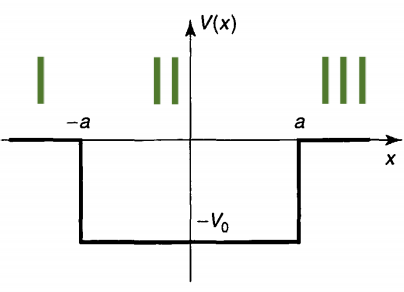
\includegraphics[width=0.3\columnwidth]{figures/finite_square_well.png}
%\end{Figure}
%\vspace{-2em}

%where $V_0$ is a positive constant.

\textit{\underline{Bound states}}: \\
%Potential is piecewise and discontinuous, can split into regions. \\

\textbf{\textit{REGION I}}
$-\frac{\hbar}{2m} \dv[2]{\psi}{x} = E \psi, \textrm{ or } \psi''_{I}(x) - \kappa^2 \psi_{I}(x) = 0, \quad \kappa \equiv \sqrt{-\frac{2mE}{\hbar}}$
where $E < 0$ for a bound state. 
General sol: $\psi_{I}(x) = Ae^{-\kappa x} + B e^{\kappa x}$. \\
$x = -\infty \rightarrow \psi(x) = 0$, so $A = 0$, and we have $\psi_{I}(x) = Be^{\kappa x}$

\smallskip

\textbf{\textit{REGION II}}
$-\frac{\hbar^2}{2m} \dv[2]{\psi}{x} - V_0 \psi = E \psi, \textrm{ or } \psi'' = -l^2 \psi, \quad l \equiv \sqrt{\frac{2m (E + V_0)}{\hbar}}$

General sol: $\psi(x) = C \sin(lx) + D \cos(lx)$, for $-a < x < a$

\smallskip

\textbf{\textit{REGION III}} 
$x = \infty \rightarrow \psi(x) = 0$, so $G=0$ and $\psi_{III}(x) = Fe^{-\kappa x}$

\medskip
\hrule height 0.3pt \thinspace

\textbf{Even bound states}:
$\psi(-x) = \psi(x)$, $\psi_{II}(x) = D \cos(lx)$ \\
Bc the potential has only a finite discontinuity at $x = \pm a$, both $\psi$ and $\psi'$ must be continuous at $x = \pm a$.

$x = a$, $\psi_{II}(a) = \psi_{III}(a)$ imposes $D \cos(la) = F e^{-\kappa a}$ \\

$x = a$, $\psi'_{II}(a) = \psi'_{III}(a)'$ imposes $-lD \sin(la) = -\kappa F e^{-\kappa a}$ \\

Continuity of $\psi(x)$ and $\psi'(x)$ at $x = -a$ does not add anything new. \\

Dividing the above two, we get $\kappa = l \tan(la)$ \\
This is a formula for the allowed energies, since $\kappa$ and $l$ are both functions of $E$. Let $z \equiv la$, and $z_0 \equiv \frac{a}{\hbar} \sqrt{2m V_0}$. $\kappa^2 + l^2 = 2m V_0 / \hbar^2$, so $\kappa a = \sqrt{{z_0}^2 - z^2}$. \\

Transcendental eq for $z$ (and hence $E$) as a function of $z_0$ (which is a measure of size of well): $\tan z = \sqrt{(\frac{z_0}{z})^2 - 1}$

\textbf{Odd bound states}
$\psi_{II}(x) = C \sin(lx)$

$x = -a, \psi_{II}(-a) = \psi_{I}(-a)$ imposes $C \sin(la) = B e^{-\kappa a}$ \\
$x = -a, \psi'_{II}(-a) = \psi'_{I}(-a)$ imposes $l C \cos(la) = -\kappa B e^{-\kappa a}$ \\

Dividing, $l \cot(la) = -\kappa$. 
In terms of $z$ and $z_0$, $\cot(z) = - \sqrt{(\frac{z_0}{z})^2 - 1}$

$V_{1}$ does not support an odd bound state, since there is no intersection pt, $V_{2}$ produces only one bound state, and $V_{3}$ produces two bound states. Finite well potential supports at least one even state, the ground state, and it may not support any of the excited states.

% \vspace{0em}
% \begin{Figure}
%     \raggedright
%     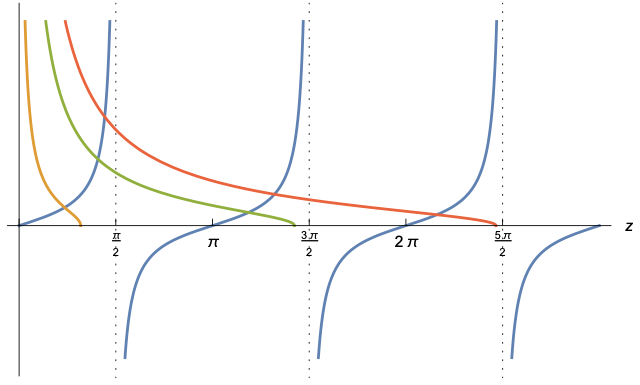
\includegraphics[width=0.4\columnwidth]{figures/even_finite_square_well.png}
% \end{Figure}
% \vspace{-1em}

% \vspace{-8em}
% \begin{Figure}
%     \raggedleft
%     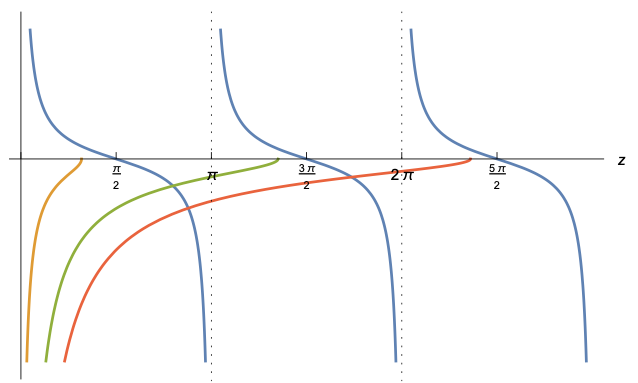
\includegraphics[width=0.4\columnwidth]{figures/odd_finite_square_well.png}
% \end{Figure}
% \vspace{-1em}

% \medskip
\hrule height 0.3pt \thinspace

\textbf{Wide and deep well}:
$z_n \approx \frac{n \pi}{2}, n = 1, 2, 3, ..., \quad E_n = -V_0 + \frac{\hbar^2 \pi^2 n^2}{2m(2a)^2}, n = 1, 2, ...$

Thus, the energy levels of the infinite square well of width $2a$ are reproduced for $E_n - (-V_0) = E_n + V_0$, which is the energy above the bottom of the well. As $V_0 \rightarrow \infty$, finite sq well goes to infinite sq well.

%\columnbreak

%\vspace{-1em}
%\begin{Figure}
% \raggedright
% 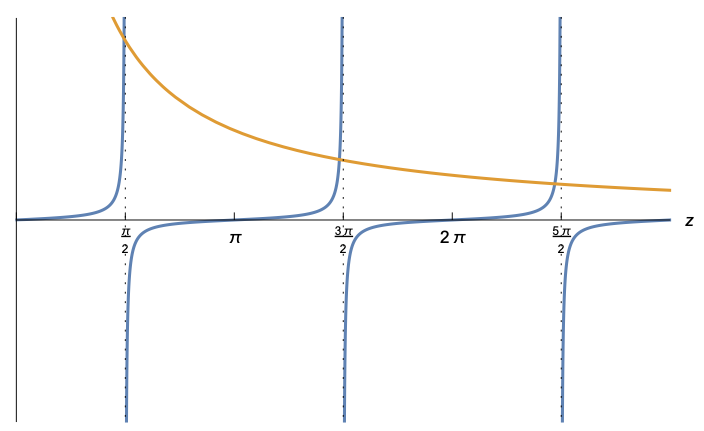
\includegraphics[width=0.3\columnwidth]{figures/wide_deep_finite_square_well.png}
%\end{Figure}
%\vspace{-1em}

%\end{vwcol}

\textbf{Shallow and narrow well}
Need $z_0 = \sqrt{\frac{2mV_0 a^2}{\hbar^2}} \geq \frac{\pi}{2}$ to support any odd state.

%\subsection{\underline{Gaussian integrals}}
%$$\int_{-\infty}^{\infty} e^{-ax^2} dx = \sqrt{\frac{\pi}{a}} \textrm{ and } \int_{0}^{\infty} e^{-ax^2} dx = \frac{1}{2} \sqrt{\frac{\pi}{a}}$$
%$$\int_{-\infty}^{\infty} x^{2n+1} e^{-ax^2} dx = 0 \textrm { for } n = 0, 1, 2, ...$$
%$$\int_{-\infty}^{\infty} x^{2n} e^{-ax^2} dx = (-1)^n \dv[n]{}{a} \sqrt{\frac{\pi}{a}} \textrm{ for } n = 0, 1, 2, ...$$
%$$\int_{-\infty}^{\infty} e^{-ax^2 + bx} dx = \sqrt{\frac{\pi}{a}} e^{\frac{b^2}{4a}}  \qquad  \int_{-\infty}^{\infty} x^n e^{-ax^2 + bx} dx = \dv[n]{}{b} \sqrt{\frac{\pi}{a}} e^{\frac{b^2}{4a}}$$

